\documentclass[10pt,a4paper]{article}
\usepackage[T1]{fontenc}
\usepackage{lmodern,mathpazo}
\usepackage[margin=22mm]{geometry}
\usepackage[numbers,sort&compress]{natbib}
\usepackage{amsmath,amssymb,booktabs,tabularx,longtable,array}
\usepackage{graphicx,xurl,enumitem,microtype,placeins}
\usepackage[colorlinks=true,allcolors=black]{hyperref}
\usepackage{fancyhdr}
\graphicspath{{figures/}}
\setlist{nosep,leftmargin=*}
\setlength{\emergencystretch}{1.5em}
\lefthyphenmin=2
\righthyphenmin=3
\newcolumntype{Y}{>{\raggedright\arraybackslash}X}
\newcommand{\Simple}{\textsc{Simple}}
\newcommand{\Local}{\textsc{Local}}
\renewcommand{\thesection}{\Alph{section}}
\renewcommand{\thefigure}{\thesection.\arabic{figure}}
\renewcommand{\thetable}{\thesection.\arabic{table}}
\renewcommand{\theequation}{\thesection.\arabic{equation}}
\counterwithin{figure}{section}
\counterwithin{table}{section}
\counterwithin{equation}{section}
\pagestyle{fancy}\fancyhf{}
\fancyhead[L]{\small Fixed-reference parallel inference}
\fancyhead[R]{\small Supplementary material}
\fancyfoot[C]{\thepage}
\setlength{\headheight}{14pt}
\hypersetup{pdftitle={Supplement: Parallelizing Quantized LLM Inference Under a Fixed Numerical Reference},pdfauthor={Chengzhan Li}}
\newcommand{\SuppApplicationRows}{%
Qwen3-8B & 2.727386 & 2.689778 & 2.728748 & 2.691337 & 2.272642 & 2.226927 \\
Qwen3-14B & 4.629760 & 4.602216 & 4.629086 & 4.602757 & 3.464285 & 3.426847 \\
Llama-8B & 2.887876 & 2.851631 & 2.887360 & 2.851517 & 2.563052 & 2.522963 \\
}

\newcommand{\SuppFactorRows}{%
8B & L\_L4\_D4/W\_L4\_D4 & 0.997913 & [0.995370, 0.999576] \\
8B & L\_P\_D4/W\_P\_D4 & 0.998717 & [0.995953, 1.000570] \\
8B & W\_P\_D4/W\_L4\_D4 & 0.983648 & [0.980236, 0.988654] \\
8B & L\_P\_D4/L\_L4\_D4 & 0.984440 & [0.981228, 0.989391] \\
8B & Interaction & 1.000696 & [1.000069, 1.001393] \\
14B & L\_L4\_D4/W\_L4\_D4 & 0.996957 & [0.994726, 0.999092] \\
14B & L\_P\_D4/W\_P\_D4 & 0.998881 & [0.997093, 1.000227] \\
14B & W\_P\_D4/W\_L4\_D4 & 0.990130 & [0.988351, 0.992804] \\
14B & L\_P\_D4/L\_L4\_D4 & 0.992041 & [0.990754, 0.993985] \\
14B & Interaction & 1.001703 & [1.000293, 1.003338] \\
}

\newcommand{\SuppPriorRows}{%
W\_REF1L\_M & 124.182883 & 7.761430 \\
W\_REF1G\_M & 117.208239 & 7.325515 \\
L\_REF1L\_M & 124.100017 & 7.756251 \\
L\_REF1G\_M & 117.143582 & 7.321474 \\
W\_REF1L\_D4 & 147.748374 & 9.234273 \\
L\_REF1G\_D4 & 133.543739 & 8.346484 \\
}

\newcommand{\SuppAmpereRows}{%
W\_L4 & 12.038851 & 13.824167 \\
W\_P & 11.897263 & 13.598468 \\
L\_L4 & 11.996725 & 13.800486 \\
L\_P & 11.878694 & 13.548505 \\
}

\newcommand{\SuppMatchedRows}{%
loop4 & 248 & 0.990445 & [0.941449, 1.042653] \\
loop4 & 252 & 0.978065 & [0.952121, 1.023051] \\
packed & 248 & 0.936989 & [0.891884, 1.001187] \\
packed & 252 & 0.947566 & [0.925460, 0.977713] \\
}

\newcommand{\SuppOperatorRows}{%
Q4\_K/q4 & 0.737011 & 0.969303 & [0.957626, 0.988546] \\
Q4\_K/q32 & 0.473109 & 0.692862 & [0.680304, 0.702919] \\
Q6\_K/q4 & 0.820466 & 0.990319 & [0.962415, 1.010187] \\
Q6\_K/q32 & 0.582934 & 0.795353 & [0.747288, 0.870814] \\
}

\newcommand{\SuppSthreePhaseRows}{%
Prefill & 143.926569 & 137.984135 & $-5.942435$\\
Decode & 216.663232 & 216.689813 & $+0.026580$\\
Reset & 0.005514 & 0.005524 & $+0.000010$\\
Planning & 0.005186 & 0.005159 & $-0.000026$\\
Owned output copy & 0.359950 & 0.367295 & $+0.007345$\\
Unpartitioned residual & 3.871228 & 3.872933 & $+0.001706$\\
\midrule
Resident service & 364.831679 & 358.924859 & $-5.906820$\\
}

% Generated by scripts/analyze_v3_history.py; edit sources, not counts.
\newcommand{\HistoryWidthRows}{%
2 & Row-Q8\_1; MMVQ, 4 warps & 16/16 & --- \\
4 & Row-Q8\_1; MMVQ, 4 warps & 16/16 & --- \\
8 & Row-Q8\_1; MMVQ, 2 warps & 0/16 & 16/16 \\
16 & MMQ quantization and MMQ\textsuperscript{a} & 0/16 & 16/16 \\
32 & MMQ quantization and MMQ\textsuperscript{a} & 0/16 & 16/16 \\
}
\newcommand{\HistoryRepairRows}{%
Projection repair & Match & 99/128 & 198/1,920 \\
Projection + attention repair & Match & 0/128 & 0/1,920 \\
Same binary, attention repair off & Match & 99/128\textsuperscript{b} & 198/1,920\textsuperscript{b} \\
Same binary, projection repair off & Differ & --- & --- \\
}
\newcommand{\HistoryProducerRows}{%
Unchanged endpoints & 5 & Match & Match & Match & Match \\
Prealgebra 1865 and 1804 & 2 & Match & Match & Differ & Match \\
GSM8K train 1184 & 1 & Match & Differ & Differ & Differ \\
}

\begin{document}
\begin{center}
{\Large\bfseries Supplementary material}\par\medskip
{\large Parallelizing Quantized LLM Inference\\Under a Fixed Numerical Reference}\par\medskip
Chengzhan Li\par
Author-review draft, 13 November 2026
\end{center}
\noindent This supplement supplies implementation coverage, complete comparisons and reproducible source identities for the main paper. Numerical observations refer to their recorded implementations and inputs. The reconstruction accompanying this draft uses CPU analysis of public records; it adds no native qualification or model timing.

\section{Numerical contract and implementation coverage}
\label{sec:supp-contract}

\subsection{What is bound and what is checked}
The reference binds the producer as well as the consumer. In the CUDA deployment, the original prompt producer uses physical microbatch one and requests its original final output. Candidate prefill can regroup known rows when the resulting requested vector and active cache preserve that producer. The controlled SmolLM2 Vulkan append study retains its original prompt calls of up to 512 tokens and physical microbatch 128. Equal emitted-token endpoints alone do not make states produced by different schedules interchangeable.

The dense append check in \texttt{phase\_append\_requirements} requires one stream, no sliding window or shifted cells, an occupied prefix whose end and physical head equal the append position, and sufficient capacity. Existing cells must have their own logical positions and include sequence zero. The native padding is at least 256 entries. The executor additionally binds F16 K/V and a context owned by its single-sequence frontend. The sequence-membership check is not an exclusivity test for externally mutated, shared caches.

The phase executor accepts all-row or last-row output requests. With zero-based row indices these modes instantiate the main paper's set $O$ as $\{0,\ldots,q-1\}$ or $\{q-1\}$, respectively. The original released Q8 frontend reserves four output rows; its all-output gate rejects wider requests before a native call, although last-only prompt calls can be wider. S3 uses a separate 32-output reserve. An eight-output diagnostic profile likewise has its own consumer and qualification. The planner's more general requested-row flags do not expose an arbitrary sparse-output API through the evaluated frontend.

Local attention requires causal, non-Flash execution, consecutive positions, one sequence, a complete prefix-extent vector, singleton K/V streams, and no attention bias, sinks or MLA path. Its descriptor includes Q/K/V types, head dimensions and counts, and V transposition. Equal-descriptor runs are tiled to at most four query columns in the admitted layout, with K, V and mask views restricted to the required extent. A noncontiguous mask is materialized before use. The planner can check the row partition; equality of the selected kernels' arithmetic remains a backend condition. Several architecture and layout requirements are assertions rather than recoverable admission statuses.

\subsection{Projection checks and reuse}
The Q8 packed branch accepts F32 activations with Q8\_0 weights and query width 5--32. Actual multi-group packing additionally requires contiguous activations, singleton higher weight dimensions and at least eight queries. It maps complete groups to $[K,4,\lfloor q/4\rfloor]$, reshapes the outputs, and handles a remaining tail with an ordinary operation of at most four columns. Widths five through seven therefore enter this branch without constructing multiple packed groups.

The same reference binding must cover the smaller widths created by a physical cut. In the four-query example, \Simple{} sends three and one rows through the graph, while \Local{} sends four. In the eight-row prefill illustration, the physical boundary is after the seventh row; local attention uses $4+3+1$ tiles and projections use $4+4$ groups. The figure shows the grouping construction, not a newly measured workload. Preserving the full-group shape does not prove equivalence for these tails, their quantizers or the surrounding decoder operations.

The marked backend-loop4 control checks contiguous Q8\_0/F32/F32 tensors, dimensions, offset bounds and absence of fused arithmetic or indexed matrix multiplication. Its CUDA dispatcher requires actual buffers on the selected device, NVIDIA warp size 32, safe padding, and MMVQ selection for every original one-to-four-column tile. These checks precede that operator's quantizer and kernel, but occur inside a decode call; earlier graph operations can already have executed.

Packed projections have no loop4 marker. Their ordinary dispatcher can select other kernels, including a cuBLAS branch for unsuitable padded views. Falling back to an ordinary graph path is not, by itself, a reference-equivalence guarantee. The mixed Q4\_K/Q6\_K experiment has its own one-column control and is outside these Q8 marker checks.

The active graph-reuse checks compare the policy, full prefix-extent vector, head-placement key, and normal graph topology and output count. Requested row indices are refreshed as graph inputs. A structural identity helper exists in the planner header but is not the live reuse key. Accordingly, neither a helper's presence nor a cache-type tag supplies a general run-time certificate for every numerical choice.

\subsection{Output lifetime, observation and failures}
After synchronization, each requested vector is copied to storage indexed by its logical row. A later group can then reuse native scratch buffers without destroying an earlier accepted frontier. The implementation checks that a requested output exists and that the physical append endpoint is correct; it does not compare reference KV bytes online. Greedy sampling checks all vector entries for finiteness and retains the first vocabulary index on ties.

The speculative loop materializes an already emitted seed and the draft proposals, samples every requested target row, and then processes acceptance in order. With $b$ initially materialized rows and $r$ accepted proposals, it trims target and draft to length $b+1+r$. A correction or bonus token is emitted after that accepted prefix and remains unmaterialized until the next decode. On a cap or end-of-generation stop, the reported stream can end in this pending state; no extra decode is introduced solely to make KV length equal emitted-stream length.

The original capture observer selects attention and specially named nodes; its filter does not include the packed projection names. Capture is disabled during clean timing. The original state-capture call records initialization and the first commit. Each other profile must be assessed from its own capture implementation and qualification records. A native sequence export also requires extraction of active K/V before it represents the reference relation in the main paper.

The target decode loop poisons its owner on exceptions from native groups and postchecks. Trim, reset, draft, sample and diagnostic failures lie outside that catch; the command-line entry exits on failure. Assertions terminate directly. The resulting process boundary prevents another request in that worker, but does not establish recovery for a library caller that catches an exception and continues.

\subsection{Diagnostics that distinguish consumer contracts}
Two CPU diagnostics demonstrate why output and state requirements must be declared together. They use a synthetic two-layer F32 model, F16 KV, a vocabulary of 128, one CPU thread and a context capacity of 1024. They are mechanism diagnostics, not GPU qualification or performance measurements~\cite{records}.

First, a two-row call and two successive one-row calls start from identical state at history length 248. Although both operation argmax values and the next forced-continuation argmax agree, 242 of 256 output float bit patterns differ. Their final serialized active-sequence states differ in 43 bytes, and the continuation differs in 127 of 128 float bit patterns. The diagnostic does not localize the cause. It demonstrates that token agreement can coexist with different full vectors, state and subsequent computation.

Second, an eight-row operation is compared with a predefined four-plus-four reference at history lengths 248 and 252. All eight shared outputs, active state, geometry and one forced continuation agree. A restricted downstream consumer instead requires the first four vectors, retains five materialized rows, and then consumes fixed token 37. This comparison uses a four-plus-one reference and trims the wider execution to the same five-row frontier. Extra vectors are captured for diagnosis, but the fifth vector is excluded from the downstream contract before execution. It differs in 117 and 128 entries at the two histories, respectively, despite unchanged argmax; the required four outputs, retained state and forced consumer agree. Thus this restricted consumer passes while one requiring the fifth vector does not. These are explicit diagnostic schedules, not an autonomous scalar deployment reference. They establish neither natural speculative acceptance behavior nor a general qualification of an eight-output production verifier.

\subsection{Captured arithmetic paths and attention repairs}
\label{sec:supp-historical-mechanisms}
The historical RTX width study captures Qwen3-0.6B-Q8\_0 and Qwen3-8B-Q8\_0 on an RTX 5070 Ti Laptop GPU. A deterministic 32-token fixture supplies real model activations. Each model contributes layer-0 Q/K/V, attention-output, FFN gate/up/down and vocabulary projections: 16 descriptors, rather than 16 independent workloads. Replays hold each captured weight and F32 activation prefix fixed. The scalar route evaluates and concatenates single columns; the native route uses a wide two-dimensional matrix; the grouped route uses $[K,4,q/4]$ and restores column order. Recorded complete-output digests give Table~\ref{tab:history-width}~\cite{records}.

\begin{table}[htbp]
\centering\small
\caption{Native width can change arithmetic; outer grouping preserves the sampled outputs. Equality counts compare the complete operator output with same-operand scalar replay across both models. CUPTI dispatch was profiled for the eight 8B descriptors. A dash means no multi-group packed operation was constructed at that width.}
\label{tab:history-width}
\begin{tabularx}{\textwidth}{@{}rYrr@{}}\toprule
Width & Native dispatch observed on 8B & Native = scalar & Grouped four = scalar\\\midrule
\HistoryWidthRows
\bottomrule\end{tabularx}
\par\smallskip\raggedright\footnotesize
\textsuperscript{a}Stream-K fixup occurs for seven of eight traced classes; the vocabulary projection omits it. Grouped widths 8/16/32 retain row-Q8\_1 and four-warp MMVQ. Internal temporary quantized bytes were not separately captured.
\end{table}

All 16 native width-32 replays reproduce their own live captures. At the first Q projection, both models additionally have matching live scalar/native input bytes and scalar-output replay. Later operator comparisons hold their captured operands fixed; they do not reconstruct a whole scalar decoder. The historical source uses four reduction warps at native widths 1--4 and two at widths 5--8. Thus width eight can alter reduction organization even with the same activation-quantizer entry point.

The Vulkan Llama companion starts from its own stock scalar reference: Meta-Llama-3.1-8B-Instruct-Q8\_0 on B570, a CPU Llama-3.2-1B-Instruct-Q8\_0 draft, capacity 1024, F16 KV and $k=3$. A scoped F32 projection policy repairs the scalar-versus-wide activation path. Endpoints then agree, but the long development input still exposes 99 different committed vectors in each speculative layout. Combining that policy with reference attention groups removes the differences (Table~\ref{tab:history-repair}). At the diagnosed boundary, changing extent also changes V contiguity and the selected matvec kernel. This is a joint attention-path repair.

\begin{table}[htbp]
\centering\small
\caption{Projection and attention repairs are complementary in the historical Vulkan case. ``Match'' refers to emitted-token and stopping endpoints. Vector columns count differing complete vocabulary vectors. The long input is CodeContests/valid/108; each of its two speculative layouts contributes 128 committed decisions. The full audit covers three inputs and five audited arms (R, M\_PQ, M\_QB, C\_PQ, C\_QB), including the R control.}
\label{tab:history-repair}
\begin{tabularx}{\textwidth}{@{}Yp{1.7cm}rr@{}}\toprule
Configuration & Endpoints & Long input, per layout & All committed rows\\\midrule
\HistoryRepairRows
\bottomrule\end{tabularx}
\par\smallskip\raggedright\footnotesize
\textsuperscript{b}The same-binary attention-off run reproduces the projection-only trajectory across all 36 requests and 3,152 saved target/draft vectors. Its committed counts follow that recorded trajectory equality. The dash in the projection-off row means no committed-vector count is used here; its endpoint failures already distinguish it. The two layouts' 99 affected positions account for 198 differing records, not 99 across the entire audit.
\end{table}

\subsection{Producer state changes consumer compatibility}
A historical B570 Qwen3-8B/0.6B Q8 test exports the initial target state into a clean receiving context. P1 produces the prompt one token per call; P4T uses four-token calls with separately defined tails. C1 is ordinary target-only continuation; PQ and QB are the two speculative layouts with $k=1$. Table~\ref{tab:history-producer} groups all eight inputs by endpoint outcome against the same independently executed reference R. PQ and QB agree with one another on endpoints, cycles and complete vectors for all 16 input--producer pairs, yet this agreement does not imply equality with R.

\begin{table}[htbp]
\centering\small
\caption{Producer $\times$ consumer endpoint compatibility at the historical boundary-zero clean-receiver interface. Each column compares with the fixed R endpoint. Grouped rows cover all eight inputs and all 48 producer/consumer cells. ``PQ/QB'' means both layouts have the displayed outcome.}
\label{tab:history-producer}
\begin{tabularx}{\textwidth}{@{}Yrcccc@{}}\toprule
Input class & $n$ & P1 C1 & P4T C1 & P1 PQ/QB & P4T PQ/QB\\\midrule
\HistoryProducerRows
\bottomrule\end{tabularx}
\end{table}

On the two prealgebra inputs, changing the producer changes whether the speculative consumers preserve R while C1 retains the same endpoint. KV serialization and the initial full logits both change on every input; this experiment does not isolate KV alone. These boundary-zero, $k=1$ observations precede the later repairs and belong to a different contract from the capacity-4096 multi-turn implementation. The included matrix retains all individual input identities and producer-conditioned comparisons.
\FloatBarrier

\section{Workloads, numerical coverage and statistical reconstruction}
\label{sec:supp-design}
The CUDA references bind a whole-prompt caller with physical microbatch one and last-only prompt output; the controlled SmolLM2 Vulkan appends retain outer prompt calls of up to 512 tokens and physical microbatch 128. The main configurations use one dense nonwrapping sequence, F16 K/V, greedy generation and non-Flash causal attention. Known-query work uses up to 32 positions. A different model, device, producer or numerical module defines a different reference.

The historical Linux Qwen/Smol reports describe comparisons of complete requested vectors and active K/V by layer and logical position. Their geometry cases cover widths 1, 4, 8 and 32, inside and crossing prefixes, tails and the tested output masks. Natural cases exercise early and later rejection, trim, pending correction and bonus tokens, native end-of-generation, caps and reset. The Llama deployment has a separately established reference. These historical observations are retained as reported qualification, rather than an independent replay of the original native records. The 32B strong-control record directly identifies full 151,936-entry output and 64-layer active-state comparisons at its tested boundaries.

The wide-verification study initially freezes source, order and analysis before 1,024 clean timings and 128 primers. A mask-reader correction is validated offline and the completed first worker is retained without rerunning the GPU; its gap remains in the worker accounting. A later joint boundary/rollback qualification on an exposed natural root adds 1,936 full-vector and 296 active-target-KV comparisons across all eight arms. These later observations extend the checked transitions, not the diagnostic coverage of the earlier clean runs.

APPS and MATH provide the natural Qwen task identities~\cite{apps,math}. Qwen 8B and 14B share 16 roots and four sessions. Llama uses 12 roots selected after excluding previous project exposure. Each six-arm panel has two separate primer requests per worker; its 48 primers are not inference units. Four-arm factorials use four Williams rows, with 256 formal requests and 32 primers per model. The original 8B two-D4 order is fixed; its compound contrast therefore retains an order confound that the later balanced factorial does not. Model hashes, prompt IDs and orders are linked in the source index.

The 32B strong comparison uses 12 roots, six coding and six mathematics, four rounds and three arms. Its 144 measured requests each follow a matched warmup. Root-level paired log ratios are averaged equally; the bootstrap resamples the two six-root strata separately. Its primary C/B interval uses 95\% coverage and secondary G comparisons 97.5\%. Q8 application and factorial intervals use 99\% coverage for their five-comparison families. Repeated sessions travel with the root under resampling. These intervals condition on the observed sessions.

The natural multi-turn pilot uses two OpenAssistant development conversations~\cite{oasst}, two rounds and eight measured episodes. Its canonical transition does not initially retain the currently generated body as reusable KV; an earlier canonical prefix can be reused on later turns. This protocol creates less local-cut opportunity than assuming that every generated body persists. Its pooled ratio is descriptive. The dataset revision's card and license identify Apache-2.0. The package includes public timing records and diagnostic projections, including short token and text excerpts used to explain the history transition; it does not bundle the full conversation corpus.

\paragraph{Reconstruction levels.}
The supplied 8B/14B/Llama service and factorial files contain 1,568 measured timing rows. The 32B strong file includes 144 warm and 144 measured rows; the multi-turn file has eight measured episodes. The CPU routines preserve original root order, bootstrap seeds and estimands. Separate NumPy and standard-library implementations agree to $2\times10^{-12}$ in the reconstructed statistics. This tolerance concerns arithmetic in the statistical analysis, not numerical compatibility of inference. Other legacy panels supply the public numeric projections or root aggregates identified in their manifests; availability of those projections does not imply availability of all native receipts.

\section{Strong-control phase account and sensitivity}
\label{sec:supp-s3}
The S3 phase account sums the same 48 measured requests in each arm. The timers partition the resident-service clock: prefill and decode include their nested backend quantization, kernels and synchronization. Those nested activities were not separately timed. Table~\ref{tab:supp-s3-phase} shows why the service reduction is concentrated in prefill. It is descriptive accounting of the original panel, not a new set of independent phase samples.

\begin{table}[htbp]
\centering\small
\caption{S3 host-phase sums in seconds. B is the shared-quantization backend scalar loop; C exposes independent scalar groups. The difference is C minus B. These totals do not replace the equal-root primary estimator.}
\label{tab:supp-s3-phase}
\begin{tabular}{@{}lrrr@{}}\toprule
Phase & B (s) & C (s) & Difference (s)\\\midrule
\SuppSthreePhaseRows
\bottomrule
\end{tabular}
\end{table}

The primary ratio remains the exponentiated mean of twelve root-level paired log ratios, 0.984864, with its original stratified 95\% interval. A post-hoc leave-one-root-out sensitivity analysis recomputes the point estimate with equal weight across the eleven remaining roots. Its range is 0.984246--0.985561: the minimum omits \texttt{CodeContests/train/99}, and the maximum omits \texttt{CodeContests/train/173}. This exploratory check was not preregistered and supplies no new confidence interval. The complete twelve estimates are in \texttt{generated/s3\_leave\_one\_root\_out.csv}; \texttt{scripts/analyze\_v2.py} reproduces them from unchanged measured rows. The pooled service ratio, 0.983809, answers a different weighting question and remains separate from the primary result.
\FloatBarrier

\section{Complete application and component comparisons}
\begin{figure}[htbp]
\centering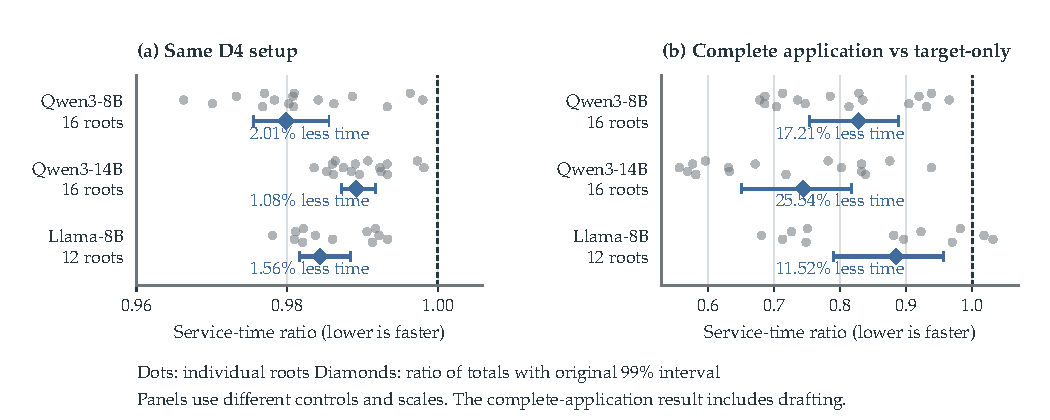
\includegraphics[width=\textwidth]{fig05_application.pdf}
\caption{The execution increment and complete speculative-application benefit. Panel (a) compares \Local-packed D4 with \Simple-loop4 D4 at the same draft setup; panel (b) compares it with the fastest measured fixed target-only M implementation. Dots sum repeated sessions within each root; diamonds are ratios of total resident time with the original 99\% paired-root intervals for five comparisons. Qwen uses 16 roots and Llama 12, each measured in four sessions. The 8B D4-arm order was fixed; the separate balanced factorial provides the stronger component attribution. The panels use separate scales.}
\label{fig:supp-application}
\end{figure}
\begin{table}[htbp]
\centering\small
\caption{Mean resident seconds per request for all six A5000 application arms. Each Qwen arm contains 64 measured requests, and each Llama arm 48. W means \Simple{} whole-graph cuts; L means \Local; L4 is backend-loop4 and P is packing. M loads target resources alone. D4 uses draft prefill microbatch four with $k=3$.}
\label{tab:supp-all-arms}
\begin{tabular}{@{}lrrrrrr@{}}\toprule
Model & W-L4-M & W-P-M & L-L4-M & L-P-M & W-L4-D4 & L-P-D4\\\midrule
\SuppApplicationRows
\bottomrule\end{tabular}
\end{table}

\begin{table}[htbp]
\centering\small
\caption{All five fixed application comparisons in each A5000 model. The numerator is L-P-D4 throughout. Each interval is a 99\% paired-root interval from that model's five-comparison family. Ratios use total resident time.}
% All five fixed application comparisons per model; generated from public timing rows.
% Requires booktabs. Numerator throughout: L_P_D4. W denotes SIMPLE.
\begin{tabular}{llrrr}
\toprule
Target & Fixed comparator & Time ratio & 99\% lower & 99\% upper \\
\midrule
Qwen3-8B & \texttt{W\_L4\_M} & 0.816506 & 0.747568 & 0.872304 \\
 & \texttt{W\_P\_M} & 0.827922 & 0.753870 & 0.888346 \\
 & \texttt{L\_L4\_M} & 0.816098 & 0.747171 & 0.872569 \\
 & \texttt{L\_P\_M} & 0.827443 & 0.753938 & 0.887542 \\
 & \texttt{W\_L4\_D4} & 0.979884 & 0.975589 & 0.985559 \\
\addlinespace
Qwen3-14B & \texttt{W\_L4\_M} & 0.740178 & 0.648295 & 0.811920 \\
 & \texttt{W\_P\_M} & 0.744608 & 0.651094 & 0.817914 \\
 & \texttt{L\_L4\_M} & 0.740286 & 0.648446 & 0.812100 \\
 & \texttt{L\_P\_M} & 0.744521 & 0.651113 & 0.817854 \\
 & \texttt{W\_L4\_D4} & 0.989193 & 0.987176 & 0.991690 \\
\addlinespace
Llama-8B & \texttt{W\_L4\_M} & 0.873640 & 0.783602 & 0.941788 \\
 & \texttt{W\_P\_M} & 0.884744 & 0.790475 & 0.956649 \\
 & \texttt{L\_L4\_M} & 0.873796 & 0.783749 & 0.941931 \\
 & \texttt{L\_P\_M} & 0.884779 & 0.790486 & 0.956653 \\
 & \texttt{W\_L4\_D4} & 0.984359 & 0.981680 & 0.988452 \\
\bottomrule
\end{tabular}

\end{table}

\begin{table}[htbp]
\centering\small
\caption{All four factorial effects and the interaction in each Qwen model. Direct effects are ratios of total service; the interaction is an equal-root geometric ratio of ratios. Intervals are 99\% paired-root percentiles in the five-comparison family.}
\begin{tabular}{@{}llrl@{}}\toprule
Model & Comparison & Ratio & Interval\\\midrule
\SuppFactorRows
\bottomrule\end{tabular}
\end{table}

\begin{table}[htbp]
\centering\small
\caption{Lifecycle costs for selected fixed controls. Resident, burst and worker clocks overlap and must not be added. A dash is an omitted field, not a zero. Workers include loading, integrity checks and primers; OS file caches were not cleared, so these are not cold-start latency claims.}
\begin{tabularx}{\textwidth}{@{}p{2.6cm}p{2.6cm}rrY@{}}\toprule
Deployment & Comparison & Resident (s) & Worker (s) & Interpretation\\\midrule
A5000 Qwen3-8B & W-P-M / L-P-D4 & 172.146 / 142.523 & 200.739 / 168.973 & Published worker totals are rounded to milliseconds.\\
A5000 Qwen3-14B & W-P-M / L-P-D4 & 294.542 / 219.318 & 662.546 / 594.559 & Measured-request bursts are 294.632 / 219.405\,s.\\
A5000 Llama-8B & L-P-M / L-P-D4 & 136.873 / 121.102 & 361.717 / 368.822 & The fastest M worker is W-P-M at 355.730\,s, a different arm from fastest resident M.\\
Windows Qwen3-8B & W-P-M / L-P-D4 & 219.810 / 155.814 & 260.240 / 192.568 & Separate deployment; input identities later reused on A5000.\\\bottomrule
\end{tabularx}
\end{table}

The Windows practical comparison gives 29.11\% less resident time and 26.00\% less worker time than the fastest fixed M. It includes the complete speculative application. Its phase account saves 96.889\,s of target work, adds 31.931\,s of draft work and 0.962\,s of other costs, for 63.996\,s net resident savings. Device-memory samples show an additional 0.705\,GiB peak for the draft-containing configuration; per-process memory peaks and energy were not measured.

The B570 resident pilot instead favors ordinary generation. Its four exposed roots and two blocks give mean times of 1.1503\,s for M and 1.8235\,s for the fastest speculative arm. A separate mechanism record has 578 local and 582 whole target graphs for 1,156 target rows, compared with 992 scalar M graphs/rows. A distinct synchronized two-root cost diagnostic saves 0.466681\,s in target work but adds 1.923330\,s in draft work and 0.210582\,s elsewhere. The different windows are not combined.

\begin{figure}[htbp]
\centering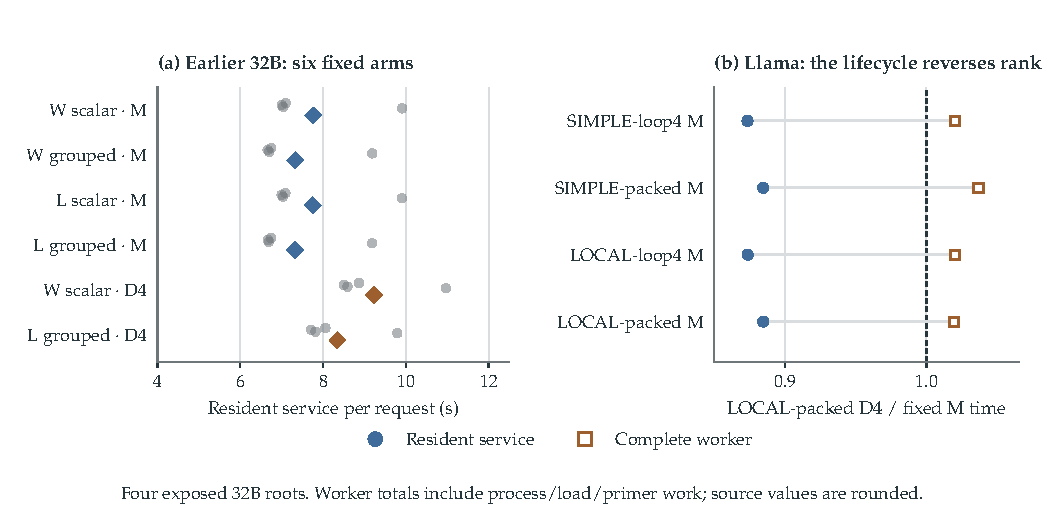
\includegraphics[width=\textwidth]{supp04_prior32b_lifecycle.pdf}
\caption{Earlier mixed-Q4 application results and the lifecycle reversal. Panel (a): the four-root 32B panel uses a graph scalar-loop control and is distinct from the later 12-root strong-backend study; all six paths are shown, including the slower speculative arms. Panel (b): Llama-8B resident and worker costs are shown for the four fixed M controls and the candidate; overlapping clocks are not stacked. Source values are public numeric projections, identified in the manifest.}
\label{fig:supp-old32}
\end{figure}

\begin{table}[htbp]
\centering\small
\caption{All six earlier Qwen3-32B mixed-Q4 arms: four exposed mathematics roots, four rounds, 16 measured requests per arm and 16 identical-root warmups. REF1L is the graph scalar-column loop and REF1G is independent grouping. The subsequent strong B control is absent from this earlier panel.}
\begin{tabular}{@{}lrr@{}}\toprule
Arm & Resident sum (s) & Mean (s)\\\midrule
\SuppPriorRows
\bottomrule\end{tabular}
\end{table}

Grouping improves this earlier panel by 5.62\% with whole cuts and 5.61\% with local cuts relative to its graph-loop control. Those effects include shared-quantization advantages that the main paper's stronger B control already obtains. Grouped D4 is 14.00\% slower than the fastest ordinary grouped arm. The strong-control operator follow-up separately uses three paired blocks in four exposed tensor cells, with one warmup and one measured operation per fresh worker. Table~\ref{tab:supp-s2} retains all cells, including mixed directions for Q6\_K/$q=4$.

\begin{table}[htbp]
\centering\small
\caption{Strong scalar-loop operator follow-up. B/G and C/B are geometric means of three paired elapsed-time ratios; ranges show observed paired minima and maxima, not confidence intervals. Equal-cell geometric ratios are 0.6390 and 0.8528. These are operator observations, distinct from the later complete service result.}
\label{tab:supp-s2}
\begin{tabular}{@{}lrrl@{}}\toprule
Cell & B/G & C/B & C/B range\\\midrule
\SuppOperatorRows
\bottomrule\end{tabular}
\end{table}
\FloatBarrier

\section{Natural-history reuse and source-derived work}
\label{sec:supp-history}
The natural two-turn pilot uses Qwen3-8B Q8 on the A5000 with capacity 4096, F16 K/V, two CPU threads and a 32-output reserve. Both arms retain backend-loop4 projections and target-only generation. The resident request timer includes reset, history rendering and tokenization, controller transport and durable per-decode accounting in the frozen host adapter. It excludes model loading, network and human waiting time, and post-response audit. These boundaries describe the experimental adapter rather than a production latency target.

The second request must reconcile its canonical history with the first request's materialized state. Table~\ref{tab:supp-history} follows the two observed transitions. The current assistant prompt ends with a four-token empty-think stub. After a capped 128-token reply, 127 body tokens are materialized and the final emitted token is pending. The next request's canonical history omits the stub, retaining the same 128 body token IDs at earlier positions. The first differing token is therefore at the start of the stub. Trimming to that common prefix is correct; reusing the old body KV would preserve the wrong positions and conditioning.

\begin{table}[htbp]
\centering\small
\caption{A timeline of the two observed history transitions. Positions are zero-based; ranges are half-open. C0 and C1 are the two free-generation conversations, not the separate supplied-history corpus. The same reconciliation is used by \Simple{} and \Local.}
\label{tab:supp-history}
\begin{tabularx}{\textwidth}{@{}p{3.7cm}p{2.2cm}p{2.2cm}Y@{}}\toprule
Transition & C0 & C1 & State consequence\\\midrule
Initial prompt, including stub & 92 tokens & 27 tokens & Four-token stub precedes the generated body.\\
After 128 emitted body tokens & KV end 219; pending 219 & KV end 154; pending 154 & The final emitted token is not yet in KV.\\
Canonical history removes stub & Body $[88,216)$ & Body $[23,151)$ & All 128 body token IDs match; their positions and prefix change.\\
Reconcile at common prefix & Keep 88; trim 131 & Keep 23; trim 131 & Remove four stub rows and 127 materialized body rows.\\
Prefill the next canonical suffix & $250-88=162$ rows & $551-23=528$ rows & Both arms recompute the required suffix before continuing.\\\bottomrule
\end{tabularx}
\end{table}

The two arms retain the same reusable earlier prefix. On later requests, older assistant turns that are already canonical can remain before the first difference. A separate CPU calculation over supplied histories predicts that 331 of 1,127 later nodes retain an earlier canonical assistant span. This is a conditional prediction for those supplied histories, not a frequency measured from free generation or a GPU saving.

The eight timed episodes sum to 36.385331\,s for whole-graph cuts and 37.920656\,s for \Local. Of the 1.535324\,s pooled difference, 1.419701\,s lies in the common sampling span. The equal-partition controls also include slower \Local{} episodes. With two conversations and two rounds, these observations do not isolate a stable local-cut penalty; they show why a saved outer call cannot by itself predict the resident result.

The proposed 89-row append provides a complementary, source-derived account. Starting at head 232, whole-call chunks are $[24,32,32,1]$ and local-call chunks $[32,32,25]$. Both retain the same ordered 23 projection tiles per fully consumed projection and 23 attention tiles per layer. Logical F32 mask storage rises from 157,696 to 182,272 bytes, while attention concatenation nodes increase from 19 to 20 per layer. The local construction additionally entails six strided-mask contiguous-copy nodes per layer, representing 24,576 logical bytes. These counts describe graph construction; actual launches, graph reuse, allocation, DRAM traffic and latency were not measured for this proposed case. \texttt{analyze\_v2.py} checks the row and tile correspondence in the fixed source analysis.
\FloatBarrier

\section{Wider execution and workload cost}
The Windows equal-work panel uses one APPS and three GSM8K origins~\cite{gsm8k}, fixed initial state, the same eight known tokens and all eight requested outputs. Its 128 measured operations and 32 primers address operation efficiency. The separate live panel uses 16 roots, prompt length at most 192, cap 96, and eight balanced order rows. Both $k=3$ and $k=7$ reserve eight outputs; 1,024 measured requests and 128 primers cover eight arms. The four primary width comparisons use 98.75\% paired-root intervals; secondary fixed-$k=7$ comparisons form a separate family.

\begin{figure}[htbp]
\centering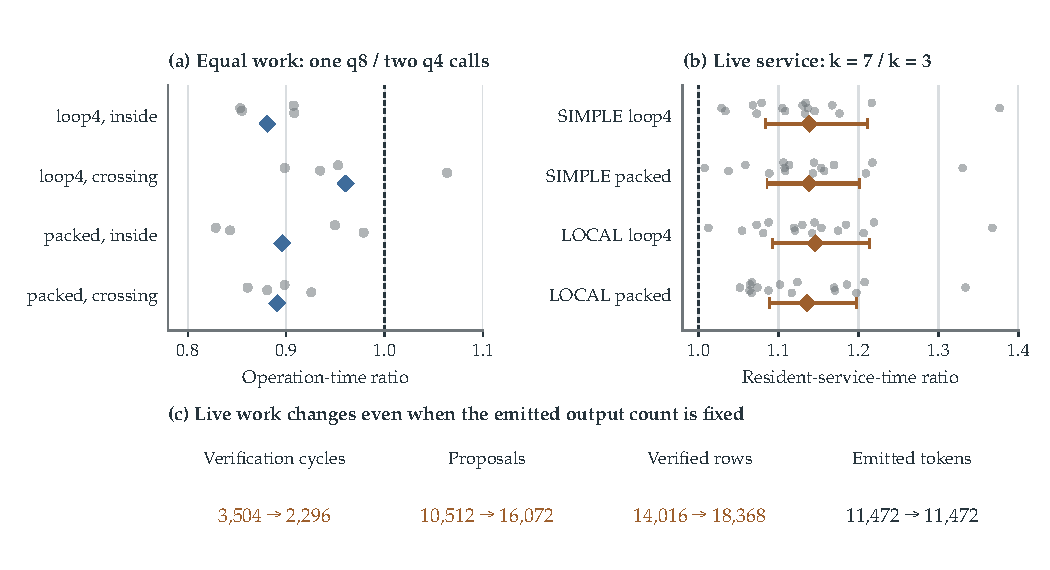
\includegraphics[width=\textwidth]{supp01_width_tradeoff.pdf}
\caption{Physical execution width and live proposal width. Equal-work $q=8$ versus two $q=4$ operations is a fixed-input comparison; $k=7$ versus $k=3$ resident generation changes the work. The live summaries use ratios of totals and 98.75\% paired-root intervals over 16 roots, with repeats clustered by root. Per-arm work counts are shared by the four methods at each $k$. These panels have different measurement boundaries.}
\end{figure}

Each live arm emits 11,472 tokens. For $k=3$/$k=7$, proposed tokens are 10,512/16,072, accepted proposals 7,928/9,152, first inspected mismatches 1,136/1,256, and unconsumed suffix tokens 1,448/5,664. Native cap/end-of-generation counts are 104/24 in each arm. Suffix waste includes post-rejection and terminal-boundary work; the aggregate counts do not separate these causes.

\begin{figure}[htbp]
\centering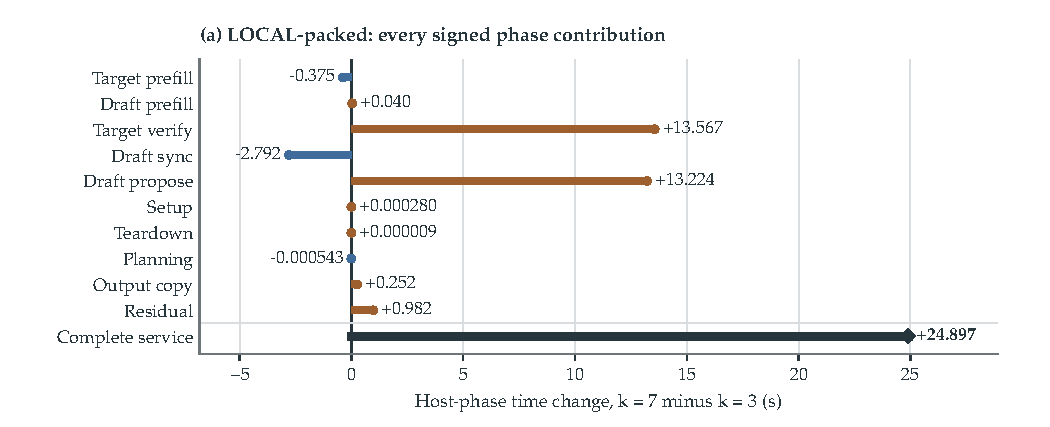
\includegraphics[width=\textwidth]{supp02_width_cost.pdf}
\caption{Where the extra live cost arises. Disjoint phase differences for \Local-packed are $k=7$ minus $k=3$ over 128 requests. Negative components save time; the net increase is 24.897\,s. Phase timers include their specified host work, synchronization and GPU execution; the residual closes the recorded service sum. These are complete-arm phase sums, not new native measurements.}
\end{figure}

The A5000 four-root pilot has 64 live measurements and 32 primers. Its \Local-packed $k=7/k=3$ ratio is 1.140572. At fixed \Local{} and $k=7$, packing/loop4 is 0.981741. A separate proposal-tape replay excludes draft work and has different target-row counts between widths, so it is not a complete-generation comparison.

\begin{table}[htbp]
\centering\small
\caption{A5000 live-width pilot. Entries are resident totals over four exposed roots and two rounds; no population interval is inferred.}
\begin{tabular}{@{}lrr@{}}\toprule
Cut / projection & $k=3$ (s) & $k=7$ (s)\\\midrule
\SuppAmpereRows
\bottomrule\end{tabular}
\end{table}

An initial A5000 equal-work comparison had unmatched first-use histories. The subsequent comparison uses 16 fresh processes, each with four warm and four measured operations, and balanced ABBA/BAAB preparation histories. It holds one exposed input, initial state and eight outputs fixed at two prefix coordinates. The complete 128-operation account gives the four process-level summaries below; mixed directions remain visible.

\begin{table}[htbp]
\centering\small
\caption{Matched-history A5000 equal-work comparison. Each cell has four fresh processes on one input; q8/q4-pair geometric means and observed process ranges are descriptive.}
\begin{tabular}{@{}lrrl@{}}\toprule
Projection & Prefix & Geometric ratio & Process range\\\midrule
\SuppMatchedRows
\bottomrule\end{tabular}
\end{table}
\FloatBarrier

\section{Boundary counterexamples and numerical migration}
The final B570 append panel has 12 fixed cells, three paths and three paired repeats, with 108 measured operations and 108 corresponding warmups. At $q=32$ it retains the registered last-only output request. Its timer begins after valid state preparation and includes phase binding, native decode, synchronization and copying the requested vector. Caller batch preparation and state import are outside it. Earlier geometries remain relevant because a $16+16$ crossing can preserve different surrounding work from a $1+31$ crossing.

\begin{figure}[htbp]
\centering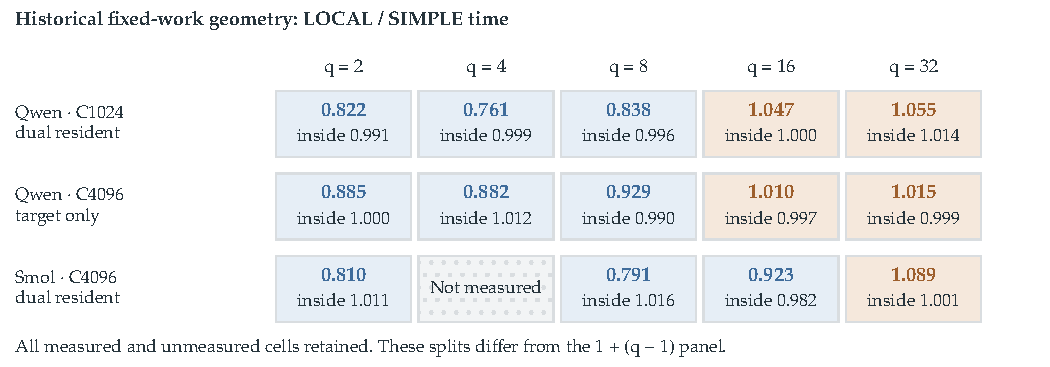
\includegraphics[width=\textwidth]{supp03_historical_geometry.pdf}
\caption{Earlier local-cut geometries, including reversals. Crossing cells are paired with inside controls; a missing cell is shown as unmeasured, not zero. These historical fixed-cell timings use their original measurement boundaries. They establish sensitivity to split geometry, not a population estimate or an isolated capacity effect.}
\end{figure}

The modern RTX comparison extracts a $4096\times4096$ Q8 projection with $q=8$ from one captured activation. U uses the upstream quantizer and few-row projection~\cite{llama_cpp_fewrow}; B retains the old reference. Table~\ref{tab:supp-rtx-variants} distinguishes the implementations. Ordinary launches with CUDA graphs disabled and the recorded programmatic-launch setting are timed using GPU events. Allocation, copies and checks are excluded; host-submission gaps can remain within an event window. The full quantization-plus-projection and projection-only boundaries have 12 paired repeats each, totaling 48 samples. Ratios are reconstructed from event duration divided by batch repetitions, avoiding rounding in the printed per-operation column.

\begin{table}[htbp]
\centering\small
\caption{Extracted RTX variants on the captured input. Register and shared-memory figures describe the projection kernel. Shared memory is per thread block; registers are per thread. No spilling is reported. C, C1 and U are measured in separate sessions against their respective B, so C/C1 is not a paired intervention. Compiler resources do not measure achieved occupancy or memory traffic.}
\label{tab:supp-rtx-variants}
\begin{tabularx}{\textwidth}{@{}p{0.65cm}Y>{\raggedright\arraybackslash}p{3.25cm}>{\raggedright\arraybackslash}p{2.5cm}r@{}}\toprule
Path & Execution change & Numerical contract & Projection resources & Complete / B\\\midrule
B & Two four-column groups in separate block groups; old packed path & Old quantizer and DP4A projection path & 63 registers; 3\,KiB static shared & 1\\
C & Two arithmetic groups in one block, reusing register-held weight fragments & Old contract, qualified on the captured case & 91 registers; 6\,KiB static shared & 1.1264\\
C1 & Sequential groups in one block, with an added barrier and no cross-group register-weight reuse & Old contract, qualified on the captured case & 64 registers; 3\,KiB static shared & 1.0261\\
U & Upstream few-row integer MMA and asynchronous weight staging & Modern quantizer and arithmetic; differs from B & 244 registers; 68\,KiB dynamic shared & 0.6129\\\bottomrule
\end{tabularx}
\end{table}

\begin{figure}[htbp]
\centering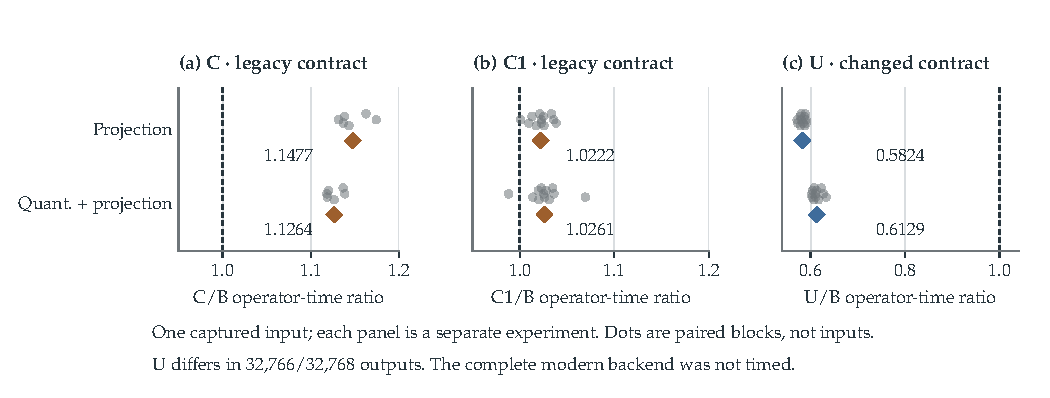
\includegraphics[width=\textwidth]{supp05_rtx_contracts.pdf}
\caption{Extracted RTX operator alternatives under distinct numerical contracts. Legacy-compatible C and C1, and modern upstream U, come from separate sessions and are not directly paired with one another. Points retain all paired repeat ratios for each boundary. U/B complete-operator time is 0.612924 with a 95\% paired-repeat interval [0.607906, 0.618665]; projection-only time is 0.582391. U does not preserve B's quantization or output bytes. The earlier old-oracle qualification failure and the unrun complete default backend have no timing point.}
\end{figure}

An earlier attempt to qualify the upstream path against a strict CPU-round-to-nearest oracle fails before timing. The subsequent study explicitly binds U's own contract and compares a valid modern numerical alternative. Static API checks for a complete current default backend pass without loading a model; full-backend numerical qualification and service timing remain unrun.
\FloatBarrier

\section{Fixed source index and access scope}
\label{sec:supp-sources}
The source package contains \texttt{data/}, \texttt{scripts/}, \texttt{figures/} and \texttt{generated/}. The figure manifests record included inputs' repository URLs, commits and SHA-256; the figure metrics record the estimands and plotted values. \texttt{build\_figures.py} produces editable SVG, vector PDF and preview PNG files. \texttt{build\_tables.py} creates editable table rows. \texttt{analyze\_v2.py} constructs the S3 phase table and post-hoc root-deletion estimates, and checks the history and 89-row source calculations. The primary CPU reconstruction scripts retain frozen seeds and reject incomplete panels. These scripts operate on public records and do not load a model or request a GPU.

Table~\ref{tab:supp-source-index} supplies direct frozen entry points. Short revision labels are hyperlinks to full commit URLs. The machine-readable manifests preserve complete identifiers and per-file hashes. An experiment revision, a source snapshot and a reconstruction revision serve different purposes and are not interchangeable.

\small
\begin{longtable}{@{}p{3.2cm}p{2.35cm}p{10.0cm}@{}}
\caption{Frozen scientific sources. Public timing records support the stated statistical reconstructions; a code or result link does not promise access to every underlying native tensor.}\label{tab:supp-source-index}\\
\toprule
Evidence & Fixed revision & Direct entry and role\\\midrule
\endfirsthead
\toprule Evidence & Fixed revision & Direct entry and role\\\midrule\endhead
\bottomrule\endfoot
Physical-range intervention & \href{https://github.com/leecdiang/HeteroSpec/blob/701079f265c0ff8fd05d43fbc2d8d5054a711e1b/platforms/rtx_reference_snapshot/benchmarks/rtx_llama_repair_v1/host_execution/RESULTS.md}{\texttt{701079f2}} & Fixed one-query AV crop/pad replay; complete operator output comparisons, with native input identity reported. Raw tensor archives were not replayed in this reconstruction.\\
Native grouping planner & \href{https://github.com/leecdiang/HeteroSpec/blob/ad16a13d2510363bb6f7c7b99241fe9ef1b54bb0/src/reference_batching/reference_batching.hpp}{\texttt{ad16a13d}} & Dense-cache requirements, physical groups and structural helper. The live graph-reuse key is separately implemented in native code.\\
Original execution sources & \href{https://github.com/leecdiang/HeteroSpec/releases/download/tpds-phase1-rtx-review-v2-evidence-20261107/rtx-phase1-source.zip}{Source snapshot} & Published source snapshot; SHA-256 begins \texttt{57cbfbfe43ae1c4b}. It identifies frontend ownership, native local attention and packed/loop4 implementations. Full hash and member identities are in the method source map.\\
32B strong-control code & \href{https://github.com/leecdiang/HeteroSpec/tree/ab695a766d055f7d3c6b1fed0720c579c749bcdb/benchmarks/server_expansion_v1/strong_baseline_followup_20261110/F0_DATA}{\texttt{ab695a76}} & Graph and MMVQ source differences for G, B and C; frozen scalar arithmetic and shared-quantization control.\\
32B service result & \href{https://github.com/leecdiang/HeteroSpec/tree/ab695a766d055f7d3c6b1fed0720c579c749bcdb/benchmarks/server_expansion_v1/strong_baseline_followup_20261110/RESULTS_S3_20261112}{\texttt{ab695a76}} & Qualification scope, reconstructed timing rows, per-root ratios, statistical report and independent reconstruction. Main strong-baseline figure and 1.51\% claim.\\
Public timing reconstruction & \href{https://github.com/leecdiang/HeteroSpec/tree/10fc03ed59e260a290a8ca8d6670d30d50f08118/benchmarks/jpdc_closeout_20261113}{\texttt{10fc03ed}} & Complete public Q8 timing rows, plans, service projections and CPU recomputation scripts. Source of the included \texttt{data/closeout/} files.\\
8B service & \href{https://github.com/leecdiang/HeteroSpec/tree/592abdfe9267fd97ecbde18cd0ee9a1bfc319e20/benchmarks/linux_transfer_v1/results_ampere_20261107}{\texttt{592abdfe}} & Original request table, plan and six-arm result. The two speculative arms retain their fixed relative order.\\
8B factorial & \href{https://github.com/leecdiang/HeteroSpec/tree/55f501e9a93013a4b4d82cc4967e82b8d9054a81/benchmarks/server_expansion_v1/M/results_ampere_m1_20261107}{\texttt{55f501e9}} & Four-arm Williams design, requests, component effects and interaction.\\
Llama confirmation & \href{https://github.com/leecdiang/HeteroSpec/tree/ca2c769c87d9b072eb050373e571abfd616ec1fa/benchmarks/server_expansion_v1/F/results_confirmation_20261108}{\texttt{ca2c769c}} & Twelve selected roots and six-arm result; \texttt{evidence/inputs-01/MODELS.json} identifies target and draft bytes.\\
14B service & \href{https://github.com/leecdiang/HeteroSpec/tree/dbca51e565ca90242ef7a39c5a6df98c1db2ba76/benchmarks/server_expansion_v1/D14/results_complete_20261108}{\texttt{dbca51e5}} & Six-arm service and worker costs on the shared Qwen roots.\\
14B factorial & \href{https://github.com/leecdiang/HeteroSpec/tree/ca6caee2cb1cd21dbcfcf1312e500a8fbb3729a8/benchmarks/server_expansion_v1/D14/results_attribution_20261108}{\texttt{ca6caee2}} & Separately measured four-arm attribution; not pooled with the service panel.\\
Natural multi-turn pilot & \href{https://github.com/leecdiang/HeteroSpec/blob/92c47c1a49243fdb871036ff39ac33babddec04b/benchmarks/server_expansion_v1/N/free_service_retry_20261113/EVIDENCE/EPISODES.json}{\texttt{92c47c1a}} & All eight timed episodes; two development conversations, two rounds and two arms.\\
Natural-history transition & \href{https://github.com/leecdiang/HeteroSpec/blob/ef1b6427b7f3b6b7d62c4249933b33b8f810d89f/benchmarks/server_expansion_v1/N/resident_opportunity_20261113/RESULTS/REPORT.json}{\texttt{ef1b6427}} & Two actual free-history reconciliations and the separate supplied-history CPU prediction; source of the timeline.\\
Proposed phase analysis & \href{https://github.com/leecdiang/HeteroSpec/tree/750346a149da58aa94a0d16016f5c451221008f7/benchmarks/server_expansion_v1/N/local_cost_decision_20261113}{\texttt{750346a1}} & Source-derived 89-row example and local-cost decision; no new service timing.\\
Controlled B570 appends & \href{https://github.com/leecdiang/HeteroSpec/tree/62f2e3345b25b59268cc2b3c131fd5ed8c7d5f88}{\texttt{62f2e334}} & Twelve geometry cells with paired inside controls; the included public projections preserve all measured cells.\\
Wide-query study & \href{https://github.com/leecdiang/HeteroSpec/tree/ba5b4c8e01d50d4bfaab1ac3908f798347be063a}{\texttt{ba5b4c8e}} & Equal-work and live-width studies, 128 root/arm aggregates, phase sums and workload counts.\\
Matched-history width & \href{https://github.com/leecdiang/HeteroSpec/tree/ab695a766d055f7d3c6b1fed0720c579c749bcdb/benchmarks/server_expansion_v1/strong_baseline_followup_20261110/RESULTS_B2_20261110}{\texttt{ab695a76}} & All 128 warm/measured operations and process-level reconstruction for four fixed cells.\\
CPU consumer diagnostics & \href{https://github.com/leecdiang/HeteroSpec/tree/af436df989570ad882db65bd8a4b265b9e8cfdae/benchmarks/frontier_cost_v1}{\texttt{af436df9}} & Synthetic CPU width and frontier diagnostics, sources and public result summaries. These diagnose output/state distinctions, not GPU performance.\\
Implementation coverage & \href{https://github.com/leecdiang/HeteroSpec/blob/10fc03ed59e260a290a8ca8d6670d30d50f08118/benchmarks/jpdc_closeout_20261113/GUARANTEES.zh.md}{\texttt{10fc03ed}} & Source-based account of online checks, capture observation, packed-node differences and failure boundaries.\\
Legacy-compatible RTX C & \href{https://github.com/leecdiang/HeteroSpec/blob/ba019f30522352c87cac2cc527082ecc6c73ed97/benchmarks/rtx223_e08_q8_20261113/numeric-v1/TIMING_SAMPLES.csv}{\texttt{ba019f30}} & All timing samples for the first extracted candidate; complete-operator C/B is 1.1264.\\
Legacy-compatible RTX C1 & \href{https://github.com/leecdiang/HeteroSpec/blob/304dcbff6d17461237774464c67ce8cb0ed60189/benchmarks/rtx223_e09_c1_20261113/ALL_SAMPLES.csv}{\texttt{304dcbff}} & Separate-session candidate timings; complete-operator C1/B is 1.0261.\\
Earlier U-oracle check & \href{https://github.com/leecdiang/HeteroSpec/blob/01a4cf847bfc8340321564c66132680d4131bf0d/benchmarks/rtx223_e10_fewrow_20261113/RESULT.json}{\texttt{01a4cf84}} & Qualification against the strict CPU-round-to-nearest oracle fails; no timing under that oracle.\\
Modern-contract U operator & \href{https://github.com/leecdiang/HeteroSpec/tree/a6a92fb08678696fdaefa4904f942237b4d3c84f/benchmarks/rtx223_e11_u_contract_20261113}{\texttt{a6a92fb0}} & Contract, wrapper, oracle, all 48 samples and analysis for the extracted modern alternative.\\
Default backend status & \href{https://github.com/leecdiang/HeteroSpec/blob/d240c5b43a763d5b02b5a53169b07f8e8af71a6c/benchmarks/rtx223_e12_backend_closure_20261113/RESULT.json}{\texttt{d240c5b4}} & Static/API result; complete backend numerical qualification and service timing are unrun.\\
Legacy numeric projections & \href{https://github.com/leecdiang/HeteroSpec/tree/e8a4981ef7db8f05cff7144fd4edc6e5a4109343/papers/reference_compatible/20261111_tpds_mainline_rewrite}{\texttt{e8a4981e}} & Earlier manuscript's \texttt{data}, \texttt{data\_added} and figure provenance preserve structural, width, lifecycle and intervention inputs. Each copied file is separately hashed.\\
\end{longtable}
\normalsize

\subsection{Public, restricted and unavailable material}
Publicly included material comprises code for reconstruction and plotting, complete timing projections for the named panels, published root aggregates, selected diagnostic summaries, and their provenance. Original model files are not bundled; their identities and upstream licenses are recorded at the linked sources. Some original native logs and tensor data are company-restricted, and some temporary intermediates were pruned. A public summary is not a substitute for an unavailable full trace. No claim is made that all original native records can be downloaded or regenerated from this document alone.

The package supports the stated CPU statistical and figure reconstruction. Running the original native experiments additionally requires the identified model bytes, hardware, numerical modules and authorized input access. The current preparation has not carried out those runs.

\bibliographystyle{unsrtnat}
\bibliography{references}
\end{document}
